\chapter{Report}
\label{cha:report}
This is a report on machine learning part.


\section{Physical Model}
Physical models are some ODEs that describe dynamic systems. The ODEs are used to generate the data that the machine learning models attempt to fit.
\subsection{Undamped Harmonic Oscillator}
Undamped harmonic oscillator is a classical hamiltonian system, in which there is no energy dissipation. The undamped harmonic oscillator can be represented by a bond-graph expression as shown in the Figure \ref{fig:undamped_harmonic_oscillator}.

\begin{figure}[h!]
    \centering
    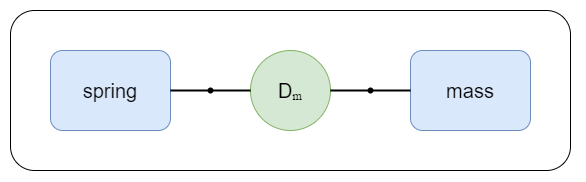
\includegraphics[scale=0.5]{figures/1_Physical_Model/1_undamped_harmonic_oscillator.png}
    \caption{Undamped harmonic oscillator}
    \label{fig:undamped_harmonic_oscillator}
\end{figure}

The total energy of the system can be represented by the Hamiltonian

\begin{equation}
    \label{eq:Hamiltonian}
    H(q,p)=q\frac{1}{2c}q+p\frac{1}{2m}p,
\end{equation}

where c is the spring compliance, q is the displacement of the spring, m is the mass, p is the momentum. The state of the system $(q,p)$ moves along the symplectic gradient

\begin{equation}
    \label{eq:symplectic_gradient}
    \dot{q}=\frac{\partial H}{\partial p}, \quad \dot{p}=-\frac{\partial H}{\partial q}.
\end{equation}

Moving along the symplectic gradient keeps the total energy of the conserve system, i.e. the Hamiltonian, constant. So that the derivative of the Hamiltonian in Equation \ref{eq:derivative_Hamiltonian} is kept as zero.

\begin{equation}
    \label{eq:derivative_Hamiltonian}
    \dot{H}=\frac{\partial H}{\partial q}\dot{q}+\frac{\partial H}{\partial p}\dot{p}=0
\end{equation}

The ODEs of the undamped harmonic oscillator are written as
\begin{equation}
    \label{eq:ODE_undamped_harmonic_oscillator}
    \begin{bmatrix}
    \dot{q}\\
    \dot{p}
    \end{bmatrix}
    =
    \begin{bmatrix}
    \frac{p}{m}\\
    -\frac{q}{c}
    \end{bmatrix}.
\end{equation}


\subsection{Isothermal Damped Harmonic Oscillator}
Isothermal damped harmonic oscillator is an exergetic port-Hamiltonian system(EPHS). The isothermal damped harmonic oscillator can be represented by a bond-graph expression as shown in the Figure \ref{fig:isothermal_damped_harmonic_oscillator}.

\begin{figure}[h!]
    \centering
    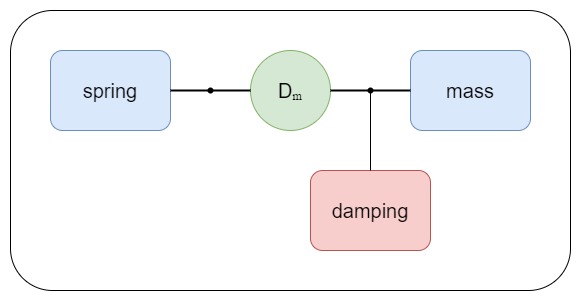
\includegraphics[scale=0.5]{figures/1_Physical_Model/2_isothermal_damped_harmonic_oscillator.png}
    \caption{Isothermal damped harmonic oscillator}
    \label{fig:isothermal_damped_harmonic_oscillator}
\end{figure}

The ODEs of the isothermal damped harmonic oscillator are written as
\begin{equation}
    \label{eq:ODE_isothermal_damped_harmonic_oscillator}
    \begin{bmatrix}
    \dot{q}\\
    \dot{p}\\
    \dot{s_{e}}
    \end{bmatrix}
    =
    \begin{bmatrix}
    \frac{p}{m}\\
    -\frac{q}{c}-d\frac{p}{m}\\
    d(\frac{p^2}{m^2})\frac{1}{\theta_{o}}
    \end{bmatrix},
\end{equation}

where $d$ is the damping coefficient, $s_{e}$ is the entropy of the environment, $\theta_{o}$ is the environmental temperature.


\subsection{Nonisothermal Damped Harmonic Oscillator}
Nonisothermal damped harmonic oscillator is an exergetic port-Hamiltonian system(EPHS). The nonisothermal damped harmonic oscillator can be represented by a bond-graph expression as shown in the Figure \ref{fig:nonisothermal_damped_harmonic_oscillator}

\begin{figure}[h!]
    \centering
    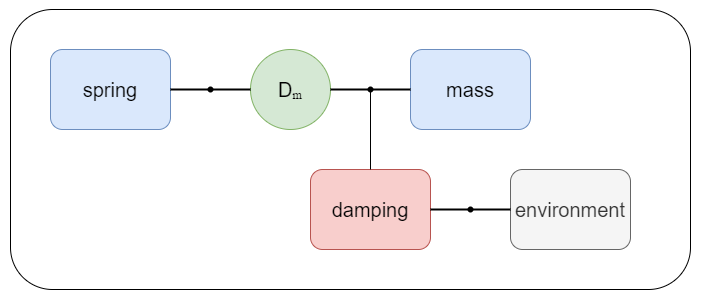
\includegraphics[scale=0.5]{figures/1_Physical_Model/3_nonisothermal_damped_harmonic_oscillator.png}
    \caption{Nonisothermal damped harmonic oscillator}
    \label{fig:nonisothermal_damped_harmonic_oscillator}
\end{figure}

The ODEs of the nonisothermal damped harmonic oscillator are written as
\begin{equation}
    \label{eq:ODE_nonisothermal_damped_harmonic_oscillator}
    \begin{bmatrix}
    \dot{q}\\
    \dot{p}\\
    \dot{s_{e}}\\
    \dot{s_{d}}
    \end{bmatrix}
    =
    \begin{bmatrix}
    \frac{p}{m}\\
    -\frac{q}{c}-d\frac{p}{m}\\
    d(\frac{p^2}{m^2})\frac{1}{\theta_{o}}\\
    \alpha(\theta_{d}-\theta_{o})/\theta_{o}
    \end{bmatrix},
\end{equation}

where $\alpha$ is the heat transfer coefficient, $\theta_{d}$ is the temperature of the damping.


\clearpage
\section{Neural ODE}
The model generated by neural ODE is considered as the baseline model. The baseline model is used to benchmark the machine learning results. \\
In hamiltonian dynamics, the states of a system $(q,p)$ are represented as points in the phase space. Let $x=[q,p]$, $dx/dt = RHS(x)$ where the RHS could be replaced with a neural network. In this case, regardless of the system, the neural network always tries to approximate the system without any physics priors.


\subsection{Undamped Harmonic Oscillator}

\begin{figure}[h!]
    \centering
    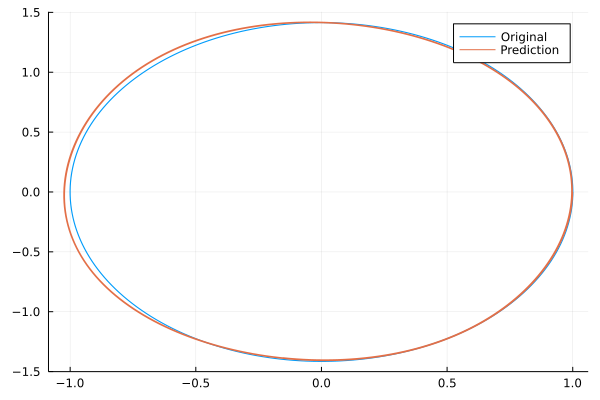
\includegraphics[scale=0.5]{figures/2_Neural_ODE/1_uho_ODE_result.png}
    \caption{Neural network prediction and origin of undamped damped harmonic oscillator}
    \label{fig:NN_ODE_udho}
\end{figure}


\clearpage
\subsection{Isothermal Damped Harmonic Oscillator}

\begin{figure}[h!]
    \centering
    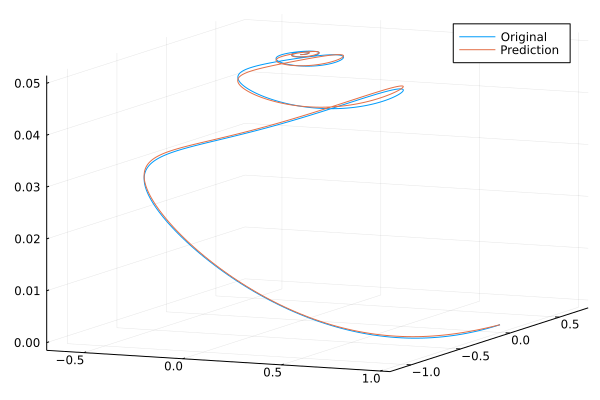
\includegraphics[scale=0.5]{figures/2_Neural_ODE/2_idho_ODE_result.png}
    \caption{Neural network prediction and origin of isothermal damped harmonic oscillator}
    \label{fig:NN_ODE_idho}
\end{figure}


\clearpage
\subsection{Nonisothermal Damped Harmonic Oscillator}

\begin{figure}[h!]
    \centering
    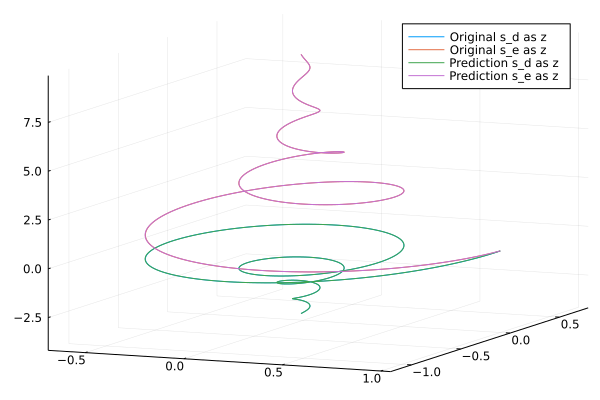
\includegraphics[scale=0.5]{figures/2_Neural_ODE/3_ndho_ODE_result.png}
    \caption{Neural network prediction and origin of nonisothermal damped harmonic oscillator}
    \label{fig:NN_ODE_ndho}
\end{figure}


\subsection{Summary of the section}
During the model training, a package called BenchmarkTools is used to print the elapsed time.

\begin{table}[h!]
	\centering
	\caption{Elapsed time for models training.}
	\label{tab:elapsed_time_neural_ODE}
	\begin{tabular}{lc}
		\toprule
		System & Elapsed time \\
		\midrule
		Undamped Harmonic Oscillator & 359.386s \\
		Isothermal Damped Harmonic Oscillator & 533.470s \\
		Nonisothermal Damped Harmonic Oscillator & 826.878s \\
		\bottomrule
	\end{tabular}
\end{table}


\clearpage
\section{Structured Neural ODE}
In previous section, the baseline model learned the state of the system $(\dot{q},\dot{p})$. The whole of the RHS was seen as a neural network. However, this method requires batches of training data and very long training time. Moreover, the baseline model lacks interpretability since it is a pure black box model. Humans cannot intuitively understand how machine obtains these models. With these considerations some works use hamiltonian-based models rather than black box models.\\ Hamiltonian-based model also known as Hamiltonian Neural Networks(HNNs)\cite{SamGreydanusMiskoDzambaJasonYosinski.}. The main purpose of HNNs is to endow neural networks with physics priors.  In fact, if the system is not conserve, it has another upper-level name called physics-informed neural network\cite{MaziarRaissiParisPerdikarisGeorgeEmKarniadakis.}, which is a method to solve ODEs with neural networks, regardless of energy conservation.
\\
In this section, the learning object is the hamiltonian. To compute the loss function, the key is to compare the truth and the model's estimation of the gradient of the neural network $(\frac{\partial{H}}{\partial{p}},\frac{\partial{H}}{\partial{q}})$.
\subsection{Undamped Harmonic Oscillator}

\subsection{Isothermal Damped Harmonic Oscillator}

\subsection{Nonisothermal Damped Harmonic Oscillator}


\clearpage
\section{Parameters estimation}
It is assumed that the ODEs of the system are completely known, except for some scalar parameters. In this case, the gradient descent algorithms can be applied in parameters estimation.
\subsection{Undamped Harmonic Oscillator}

\begin{figure}[h!]
    \centering
    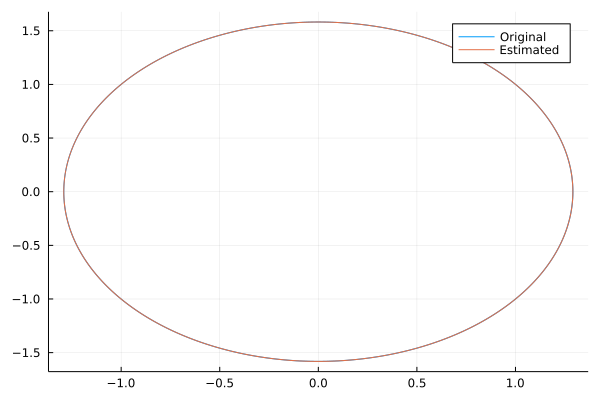
\includegraphics[scale=0.5]{figures/4_Params_Estimation/1_params_estimation_result.png}
    \caption{Parameters estimation result of undamped damped harmonic oscillator}
    \label{fig:params_est_udho}
\end{figure}


\clearpage
\subsection{Isothermal Damped Harmonic Oscillator}

\begin{figure}[h!]
    \centering
    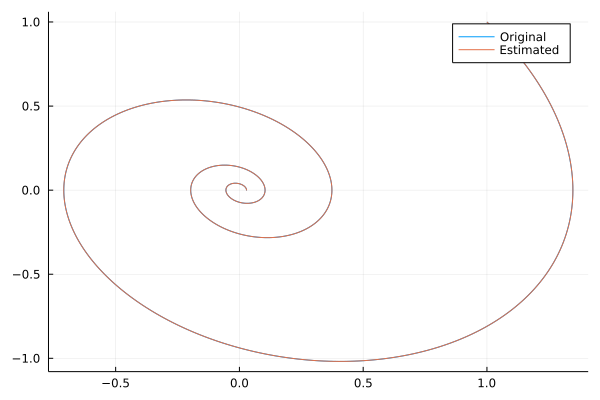
\includegraphics[scale=0.5]{figures/4_Params_Estimation/2_params_estimation_result.png}
    \caption{Parameters estimation result of isothermal damped harmonic oscillator}
    \label{fig:params_est_idho}
\end{figure}


\clearpage
\subsection{Nonisothermal Damped Harmonic Oscillator}

\begin{figure}[h!]
    \centering
    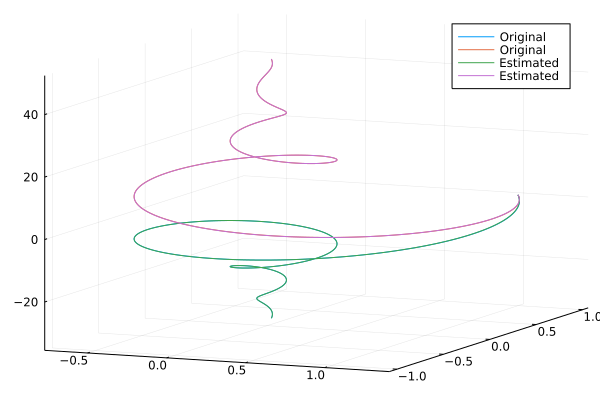
\includegraphics[scale=0.5]{figures/4_Params_Estimation/3_params_estimation_result.png}
    \caption{Parameters estimation result of nonisothermal damped harmonic oscillator}
    \label{fig:params_est_ndho}
\end{figure}

\clearpage
\subsection{Summary of the section}

\begin{table}[h!]
	\centering
	\caption{Result of parameters estimation.}
	\label{tab:result_params_estimation}
	\begin{tabularx}{\textwidth}{ll}
		\toprule
		\textbf{System 1} & \textbf{Undamped Harmonic Oscillator} \\
		\midrule
		Ground truth & [1.5, 1.0] \\
		\tabularnewline
		Estimated parameters & [1.5003, 0.99971] \\
		\tabularnewline
		Error & 0.0232\% \\
	\end{tabularx}
	
	\begin{tabularx}{\textwidth}{ll}
		\toprule
		\textbf{System 2} & \textbf{Isothermal Damped Harmonic Oscillator} \\
		\midrule
		Ground truth & [1.0, 0.4, 1.0, 1.0] \\
		\tabularnewline
		Estimated parameters & [1.0035, 0.40059, 0.99973, 0.99689] \\
		\tabularnewline
		Error & 0.264\% \\
	\end{tabularx}
	
	\begin{tabularx}{\textwidth}{ll}
		\toprule
		\textbf{System 3} & \textbf{Nonisothermal Damped Harmonic Oscillator} \\
		\midrule
		Ground truth & [1.0, 0.4, 1.0, 2.0, 3.0, 5.0] \\
		\tabularnewline
		Estimated parameters & [1.004, 0.40149, 0.9967, 2.0003, 3.0003, 5.0008] \\
		\tabularnewline
		Error & 0.0867\% \\
		\bottomrule
	\end{tabularx}
\end{table}

Error in the table \ref{tab:result_params_estimation} is computed with the formula

\begin{equation}
Error = \sqrt{\frac{RSS}{\sum_{i=1}^{m}\left(y_{i}\right)^{2}}},
\end{equation}

where $RSS = \sum_{i=1}^{m}\left(y_{i}-\hat{f}\left(x_{i}\right)\right)^{2}$ is the residual sum of squares in statistics.


